\documentclass[10pt]{article}
\usepackage{fontspec}
\setmainfont{Times New Roman}
\usepackage[russian]{babel}
\usepackage{amsmath}
\usepackage[a4paper,landscape,margin=1.3cm]{geometry}
\usepackage{graphicx,xcolor,colortbl,array,enumitem}
\arrayrulecolor[HTML]{B5B4AB}\definecolor{head}{HTML}{F0EFEC}\definecolor{ink2}{HTML}{52514E}
\setlist{nosep,leftmargin=1.3em,itemsep=0.25em}
\setlength{\parindent}{0pt}\setlength{\parskip}{0.45em}
\setlength{\tabcolsep}{4pt}\renewcommand{\arraystretch}{1.1}
\begin{document}
\selectlanguage{russian}
{\LARGE\bfseries Головы внимания MNN-Pocket-0.3B и Qwen3-0.6B: общие тенденции}\\[0.2em]
{\color{ink2} MNN-Pocket-0.3B: 28 слоёв $\times$ 14 голов $=$ 392. Qwen3-0.6B: 28 слоёв $\times$ 16 голов $=$ 448. Одна архитектура (Qwen3), один проверочный текст (WikiText-2, 8192 токена). Там, где стоят два числа, первое относится к MNN-Pocket-0.3B, второе~— к Qwen3-0.6B.}

\section*{1. Что общее}
\begin{itemize}
\item \textbf{Большинство голов смотрит по расстоянию.} По расстоянию смотрят 233 из 392 и 246 из 448 голов, дальний контекст усредняют 132 и 187, по содержанию выбирают только 27 и 15.
\item \textbf{Быстрые частоты RoPE кодируют расстояние, медленные~— содержание.} «Предыдущий токен» берёт 0,44 и 0,42 преимущества цели на частотах с периодом меньше 20 токенов. На частотах с периодом больше 20 тысяч токенов «Тот же токен» берёт 0,85 и 0,88, индукция~— 0,92 и 0,98, сток~— 0,69 и 1,00.
\item \textbf{Сток создают отдельные нейроны одного MLP.} На первом токене они срабатывают в тысячи раз сильнее обычного (3351 и 11654 раз), и норма остаточного потока там вырастает до 50 и 530 от обычной. Ключи читают эту запись на медленных частотах.
\item \textbf{Индукция собрана одинаково.} Ключ приходит из предыдущих голов, главный источник~— голова «Предыдущий токен» (у 5 из 6 и у 3 из 3 индукционных голов); запрос несёт сам текущий токен.
\item \textbf{Ширину окна задаёт крутизна позиционного ядра.} Между расстояниями 1 и 64 ядро падает на 5,3 и 5,9 логита у «Локального окна ≤ 8», на 2,8 и 3,1 у «Окна ≤ 64», на 1,1 и 0,9 у «Дальнего контекста».
\item \textbf{Чем глубже, тем меньше решает сам токен.} Он объясняет 1,00 и 0,95 запроса в слое 0, 0,60 и 0,60 в слое 5, 0,30–0,43 и 0,41–0,52 после слоя 12.
\end{itemize}
\section*{2. Чем различаются}
\begin{itemize}
\item \textbf{Сток у Qwen3-0.6B раньше и сильнее.} Его создаёт MLP слоя 2 (5 нейронов), у MNN-Pocket-0.3B~— MLP слоя 6 (1 нейрон). Приписку «+ сток» имеют 376 из 448 голов против 147 из 392; в последних десяти слоях на первый токен уходит 0,53–0,78 внимания против 0,18–0,32.
\item \textbf{Большой вес нормализации ключей работает по-разному.} У MNN-Pocket-0.3B вес 11,2 (медиана 1,9) стоит на частоте с периодом 9676 токенов и задаёт спад с расстоянием: замена на медиану поднимает долю внимания дальше 256 токенов с 0,30 до 0,63. У Qwen3-0.6B вес 96,5 (медиана 2,3) стоит на частоте с периодом 305971 токенов, но запрос на этой компоненте почти нулевой (не больше 0,02), и замена веса ничего не меняет: 0,13 → 0,17.
\item \textbf{Состав голов.} «Сам токен»: 31 (8\,\%) у MNN-Pocket-0.3B и 51 (11\,\%) у Qwen3-0.6B. «Собирает определённые токены»: 11 (3\,\%) и 0 (0\,\%).
\end{itemize}
\noindent\begin{minipage}{\linewidth}
\section*{3. Графики по слоям}
\begin{center}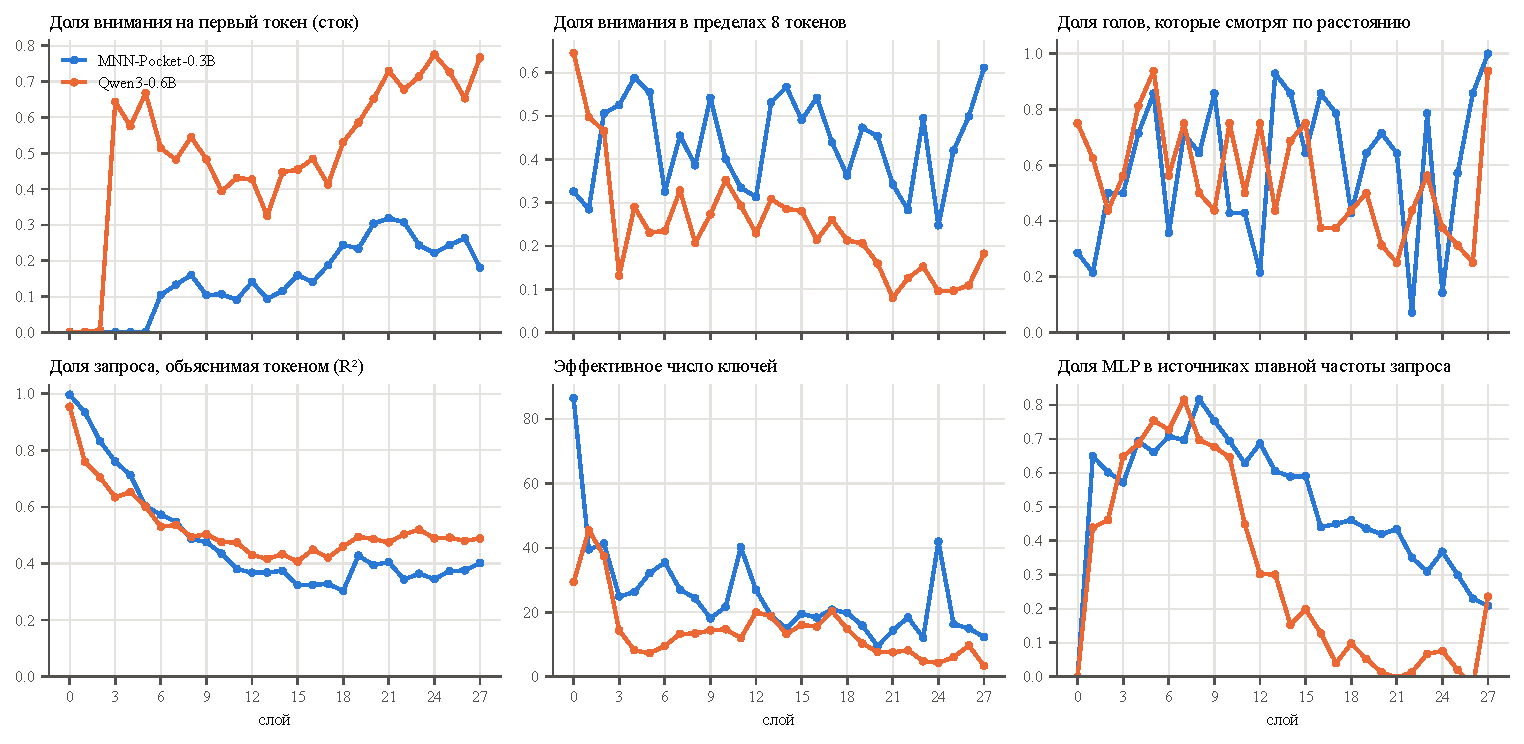
\includegraphics[width=0.9\linewidth]{heads_compare_pocket03b_06b_fig.pdf}\end{center}
\end{minipage}
\par
\noindent\begin{minipage}{\linewidth}
\section*{4. Сравнение в числах}
\begin{center}{\small\begin{tabular}{|p{11.2cm}|r|r|}\hline
\rowcolor{head}\textbf{Показатель} & \textbf{MNN-Pocket-0.3B} & \textbf{Qwen3-0.6B} \\ \hline
Слоёв $\times$ голов; групп ключей и значений & 28 $\times$ 14; 2 & 28 $\times$ 16; 8 \\ \hline
Вид «Предыдущий токен»: голов (доля) & 10 (3\,\%) & 16 (4\,\%) \\ \hline
Вид «Сам токен»: голов (доля) & 31 (8\,\%) & 51 (11\,\%) \\ \hline
Вид «Локальное окно ≤ 8»: голов (доля) & 105 (27\,\%) & 92 (21\,\%) \\ \hline
Вид «Окно ≤ 64»: голов (доля) & 87 (22\,\%) & 87 (19\,\%) \\ \hline
Вид «Тот же токен»: голов (доля) & 10 (3\,\%) & 12 (3\,\%) \\ \hline
Вид «Индукция»: голов (доля) & 6 (2\,\%) & 3 (1\,\%) \\ \hline
Вид «Собирает определённые токены»: голов (доля) & 11 (3\,\%) & 0 (0\,\%) \\ \hline
Вид «Дальний контекст»: голов (доля) & 132 (34\,\%) & 187 (42\,\%) \\ \hline
Приписка «+ сток»: голов (доля); слои & 147 (38\,\%); \mbox{6–10}, \mbox{12–27} & 376 (84\,\%); \mbox{3–27} \\ \hline
Сток: слой MLP; нейронов на 90\,\% записи; активация на первом токене относительно обычной & 6; 1; 3351 & 2; 5; 2824–11654 \\ \hline
Норма остаточного потока на первом токене относительно обычной: до и после этого MLP & 1,4 → 49,9 & 1,5 → 529,8 \\ \hline
Доля внимания на первый токен в последних десяти слоях; максимум у одной головы & 0,18–0,32; 0,40 & 0,53–0,78; 0,98 \\ \hline
«Предыдущий токен»: доля преимущества цели на частотах с периодом меньше 20 токенов & 0,44 & 0,42 \\ \hline
Доля преимущества на частотах с периодом больше 20 тысяч токенов: тот же токен / индукция / сток & 0,85 / 0,92 / 0,69 & 0,88 / 0,98 / 1,00 \\ \hline
Преимущество цели, логиты: предыдущий токен / сам токен / тот же токен / индукция / сток & $+$11,7 / $+$10,4 / $+$6,6 / $+$6,5 / $+$0,9 & $+$9,5 / $+$9,2 / $+$6,7 / $+$7,2 / $+$9,1 \\ \hline
Индукция: у скольких голов главный источник ключа~— голова «Предыдущий токен»; доля ключа из голов & 5 из 6; целиком & 3 из 3; целиком \\ \hline
Падение ядра между расстояниями 1 и 64, логиты: окно ≤ 8 / окно ≤ 64 / дальний контекст & 5,3 / 2,8 / 1,1 & 5,9 / 3,1 / 0,9 \\ \hline
Наибольший вес нормализации ключей в слое 0 (медиана); период его частоты, токенов & 11,2 (1,9); 9676 & 96,5 (2,3); 305971 \\ \hline
Доля внимания дальше 256 токенов в слое 0: исходные веса → этот вес заменён на медиану & 0,30 → 0,63 & 0,13 → 0,17 \\ \hline
Доля запроса, объяснимая токеном: слой 0 / слой 5 / после слоя 12 & 1,00 / 0,60 / 0,30–0,43 & 0,95 / 0,60 / 0,41–0,52 \\ \hline
Источники главной частоты запроса: наибольшая доля MLP в слоях 1–15; доля голов в последнем слое & 0,82; 0,79 & 0,82; 0,76 \\ \hline
\hline\end{tabular}}\end{center}
\end{minipage}
\par
\textbf{Границы сравнения.} Обе модели проверены на одном коротком тексте, виды голов определены по одним и тем же порогам. Сравнение касается того, куда головы смотрят; что они записывают в остаточный поток, сюда не входит.
\end{document}
